\documentclass{beamer}

% \usepackage[utf8]{inputenc}
\usepackage{tikz}
\usepackage{verbatim}

\usepackage{algorithm}
\usepackage[noend]{algpseudocode}


\usetheme{CambridgeUS}
\usetikzlibrary{positioning}


\begin{document}


\section{Union-Find algorithm}

\section{REM algorithm}

\begin{frame}{Inserting an edge}
  \only<1> {$p(5) > p(3)$}
  \onslide<2> {$p(2) > p(3)$}

  \begin{figure}
    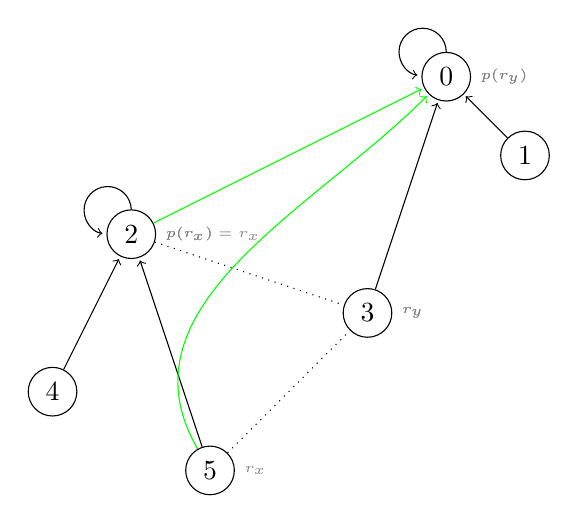
\begin{tikzpicture}[shorten >=1pt,->]
      \tikzstyle{vertex} = [circle, draw=black]
      \tikzstyle{legend} = [color=gray, font=\tiny]

      % Nodes
      \foreach \index / \x in {0/5, 1/6, 2/1, 3/4, 4/0, 5/2}
        \node[vertex] (\index) at (\x, 5-\index) {$\index$};

      % Edges
      \draw[->] (4) -- (2);
      \onslide<-2> {
        \draw [->] (2.90) arc (2:264:3mm) {} (0);
      }
      \onslide<3-> {
        \draw[green, ->] (2) -- (0);
      }

      \onslide<-1> {
        \draw[->] (5) -- (2);
      }
      \onslide<2-> {
        \draw[green, ->] [in=225, out=120] (5) to (0);
      }

      \draw [->] (0.90) arc (0:264:3mm) {} (0);
      \draw[->] (1) -- (0);
      \draw[->] (3) -- (0);

      % Edge to insert
      \onslide<1>{\draw[dotted, -] (5) -- (3);}
      \onslide<2>{\draw[dotted, -] (2) -- (3);}

      % r_x and r_y legend
      \onslide<1> {
        \node[legend, right=0mm of 5] {$r_x$};
        \node[legend, right=0mm of 3] {$r_y$};
        \node[legend, right=0mm of 2] {$p(r_x)$};
        \node[legend, right=0mm of 0] {$p(r_y)$};
      }
      \onslide<2> {
        \node[legend, right=0mm of 2] {$p(r_x) = r_x$};
        \node[legend, right=0mm of 3] {$r_y$};
        \node[legend, right=0mm of 0] {$p(r_y)$};
      }
    \end{tikzpicture}

    \caption{Inserting edge $(5, 3)$}
  \end{figure}
\end{frame}

\begin{frame}{Inserting an edge}
  \only<1> {$p(5) > p(3)$: $r_x \leftarrow p(r_x)$}
  \only<2> {$p(4) < p(3)$: $r_y \leftarrow p(r_y)$}
  \only<3> {$p(4) > p(2)$: $r_x \leftarrow p(r_x)$}
  \onslide<4> {$p(1) > p(2)$: $r_x \leftarrow p(r_x)$}

  \begin{figure}
    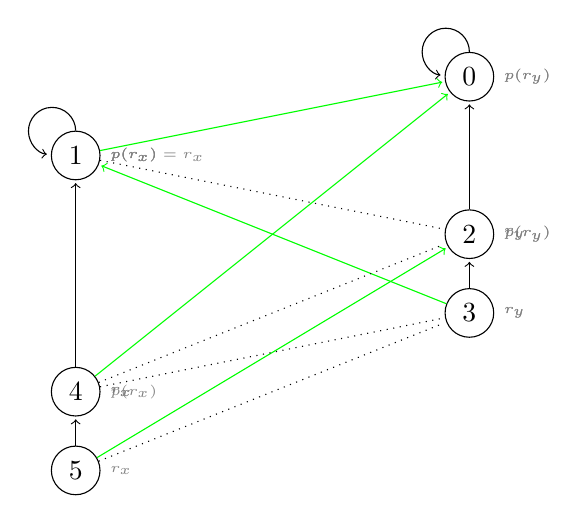
\begin{tikzpicture}[shorten >=1pt,->]
      \tikzstyle{vertex} = [circle, draw=black]
      \tikzstyle{legend} = [color=gray, font=\tiny]

      % Nodes
      \foreach \index / \x in {0/5, 1/0, 2/5, 3/5, 4/0, 5/0}
        \node[vertex] (\index) at (\x, 5-\index) {$\index$};

      % Edges
      \onslide<-4> {
        \draw [->] (1.90) arc (1:264:3mm) {} (1);
      }
      \onslide<-3> {
        \draw[->] (4) -- (1);
      }
      \onslide<-1> {
        \draw[->] (5) -- (4);
      }

      \draw [->] (0.90) arc (0:264:3mm) {} (0);
      \draw[->] (2) -- (0);
      \onslide<-2> {
        \draw[->] (3) -- (2);
      }

      \onslide<2-> {
        \draw[green, ->] (5) -- (2);
      }

      \onslide<3-> {
        \draw[green, ->] (3) -- (1);
      }

      \onslide<4-> {
        \draw[green, ->] (4) -- (0);
      }

      \onslide<5-> {
        \draw[green, ->] (1) -- (0);
      }

      % Edge to insert
      \onslide<1>{\draw[dotted, -] (5) -- (3);}
      \onslide<2>{\draw[dotted, -] (4) -- (3);}
      \onslide<3>{\draw[dotted, -] (4) -- (2);}
      \onslide<4>{\draw[dotted, -] (1) -- (2);}

      % r_x and r_y legend
      \onslide<1> {
        \node[legend, right=0mm of 5] {$r_x$};
        \node[legend, right=0mm of 4] {$p(r_x)$};
        \node[legend, right=0mm of 3] {$r_y$};
        \node[legend, right=0mm of 2] {$p(r_y)$};
      }
      \onslide<2> {
        \node[legend, right=0mm of 4] {$r_x$};
        \node[legend, right=0mm of 1] {$p(r_x)$};
        \node[legend, right=0mm of 3] {$r_y$};
        \node[legend, right=0mm of 2] {$p(r_y)$};
      }
      \onslide<3> {
        \node[legend, right=0mm of 4] {$r_x$};
        \node[legend, right=0mm of 1] {$p(r_x)$};
        \node[legend, right=0mm of 2] {$r_y$};
        \node[legend, right=0mm of 0] {$p(r_y)$};
      }
      \onslide<4> {
        \node[legend, right=0mm of 1] {$p(r_x) = r_x$};
        \node[legend, right=0mm of 2] {$r_y$};
        \node[legend, right=0mm of 0] {$p(r_y)$};
      }
    \end{tikzpicture}

    \caption{Inserting edge $(5, 3)$}
  \end{figure}
\end{frame}

\section{Distributed REM algorithm}


\end{document}
